\chapter{Priestley duality}\label{ch:priestley}

In this chapter, we show how to extend the duality for finite distributive lattices given in Chapter~\ref{ch:order} to \emph{all} distributive lattices. The two key ideas, due to Stone,\endnote{The greatly influential American mathematician Marshall H. Stone introduced Stone duality, for Boolean algebras and bounded distributive lattices in a series of papers published in the 1930s \cite{Stone1934, Stone1935, Stone1936, Stone1937BA, Sto1937/38, Sto1938BA}. Priestley duality \cite{Pri1970} recasts Stone duality in terms of Nachbin's theory of ordered spaces \cite{Nachbin64}. See also results in this direction by Nerode \cite{Ne59}.} are to generalize the join/meet-prime elements of the finite case to \emph{prime filters/ideals} (Section~\ref{sec:primefiltersideals}), and to introduce \emph{topology} on the structure dual to a distributive lattice (Section~\ref{sec:topologize}), which leads us to a dual equivalence or \emph{duality}. The main technical tool is Stone's Prime Filter-Ideal Theorem, Theorem~\ref{thm:DPF}. In this chapter we elaborate a modern variant of Stone's original duality, \emph{Priestley duality}. The precise connection between Priestley's duality and Stone's original duality will be made in Theorem~\ref{thm:Stone-isom-Priestley} in Chapter~\ref{chap:Omega-Pt}. After treating distributive lattice duality, we show in the final Section~\ref{sec:boolenv-duality} how the more widely known duality for Boolean algebras follows as an easy consequence. Throughout the chapter, in-between introducing the general concepts and proving results about them, we show how to compute dual spaces of several distributive lattices, as `running examples'. We encourage the reader to work through the examples and accompanying exercises in detail, as we believe this is crucial for developing an intuition for dual spaces.

\section{Prime filters and ideals}\label{sec:primefiltersideals}
Recall from Section~\ref{sec:finDLduality} that every finite distributive lattice can be represented by the poset of its join-irreducible elements. The following example of an infinite distributive lattice shows why join-irreducibles can not be used in general.
\begin{example}\label{exa:nojoinirr}
Consider the lattice $L = \{\bot\} \oplus (\mathbb{N}^\op)^2$, depicted in Figure~\ref{fig:nojoinirr}. Every element $(m,n)$ in this lattice is the join of the two elements $(m+1,n)$ and $(m,n+1)$ strictly below it. Therefore, there are no join-irreducibles in $L$, $\J(L) = \emptyset$.
\end{example}
\begin{figure}[htp]
\begin{center}
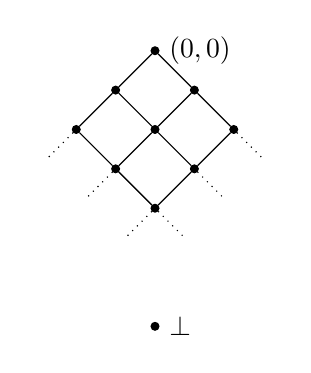
\begin{tikzpicture}
\node[draw,circle,inner sep=1pt,fill,label=right:{$(0,0)$}] (1) at (0,3) {};
\node[draw,circle,inner sep=1pt,fill] (a) at (-.5,2.5) {};
\node[draw,circle,inner sep=1pt,fill] (b) at (.5,2.5) {};
\node[draw,circle,inner sep=1pt,fill] (c) at (-1,2) {};
\node[draw,circle,inner sep=1pt,fill] (d) at (0,2) {};
\node[draw,circle,inner sep=1pt,fill] (e) at (1,2) {};
\node[] (x) at (-1.5,1.5) {};
\node[draw,circle,inner sep=1pt,fill] (f) at (-.5,1.5) {};
\node[draw,circle,inner sep=1pt,fill] (g) at (.5,1.5) {};
\node[] (w) at (1.5,1.5) {};
\node[] (y) at (-1,1) {};
\node[draw,circle,inner sep=1pt,fill] (h) at (0,1) {};
\node[] (v) at (1,1) {};
\node[] (z) at (-.5,.5) {};
\node[] (u) at (.5,.5) {};
\node[draw,circle,inner sep=1pt,fill,label=right:{$\bot$}] (0) at (0,-.5) {};
\draw[thin] (1) -- (a);
\draw[thin] (1) -- (b);
\draw[thin] (a) -- (c);
\draw[thin] (a) -- (d);
\draw[thin] (b) -- (d);
\draw[thin] (b) -- (e);
\draw[thin] (c) -- (f);
\draw[thin] (d) -- (f);
\draw[thin] (d) -- (g);
\draw[thin] (e) -- (g);
\draw[thin] (f) -- (h);
\draw[thin] (g) -- (h);
\draw[thin] (f) -- (h);
\draw[thin,dotted] (c) -- (x);
\draw[thin,dotted] (f) -- (y);
\draw[thin,dotted] (h) -- (z);
\draw[thin,dotted] (h) -- (u);
\draw[thin,dotted] (g) -- (v);
\draw[thin,dotted] (e) -- (w);
\end{tikzpicture}
\end{center}
\label{fig:nojoinirr}
\caption{A distributive lattice with no join-irreducible elements}
\end{figure}



To find the correct notion that should replace `join-irreducible' in the case of infinite distributive lattices, we need to change our perspective from specific \emph{elements} of the lattice to specific \emph{subsets} of the lattice. If $L$ is a distributive lattice and $j \in \J(L)$, then $j$ can be uniquely represented by the collection $F_j$ of elements greater than or equal to $j$. Elements of $F_j$ can be thought of as `approximations' of the element $j$, which grow in precision as one moves downward in the set $F_j$; indeed, $j$ is the infimum of this set $F_j$. In the case of infinite lattices, while join-irreducibles $j$ themselves may fail to exist (Example~\ref{exa:nojoinirr} above), these `approximating sets' $F$ will still exist. The formal notion of `approximating set' is that of a \emph{prime filter}, defined as follows.\endnote{Just as join-prime elements in a (finite) distributive lattices are a special case of join-irreducible elements in general lattice theory, the notion of prime filter in a distributive lattice can be generalized to a notion of `optimal' filter, which applies to lattices that are not necessarily distributive. Recall however from Chapter~\ref{ch:order}, note~\ref{not:nondistcase1}, that we only treat duality for distributive lattices in this book.}
\begin{definition}\index{filter}\index{filter!prime}\index{prime filter}
Let $L$ be a distributive lattice. A subset $F$ of $L$ is called a \emph{filter} if it is non-empty, an up-set, and for any $a, b \in L$, if $a \in F$ and $b \in F$, then $a \wedge b \in F$. A filter is called \emph{proper} if $F \neq L$, or, equivalently, $\bot \not\in F$. A filter $F$ is called \emph{prime} provided that $F$ is proper, and, for any $a, b \in L$, if $a \vee b \in F$, then $a \in F$ or $b \in F$.
\end{definition}
One way to think of filters in a lattice is that a filter represents an `idealized element', in much the same way as Noether's ideals in rings. In this point of view, a non-principal filter stands for a meet that does not exist in the lattice. Note that if $S$ is a subset of a lattice and $S \subseteq S'$, if infima of both sets exist, then $\bigwedge S' \leq \bigwedge S$. Thus, since taking a meet over a larger set yields a smaller element, it is natural to postulate the \emph{reverse} inclusion on filters, as we will do here. The dual notion of \emph{ideal} in a lattice is introduced in Definition~\ref{def:ideal} below; there, the order of (non-reversed) subset inclusion is the natural one, since ideals in a lattice stand for an idealized join, and taking joins over larger sets yield larger elements.


With the point of view that filters stand for idealized meets, \emph{prime} filters stand for idealized join-irreducible elements. More precisely, in finite lattices, prime filters are in one-to-one correspondence with join-prime elements: to any join-prime element $j$, one may associate the prime filter $F_j := {\uparrow}j$ of elements greater than or equal to $j$ (Exercise~\ref{exe:joinprime-primefilt}). Notice that, also here, $j \leq j'$ if, and only if, $F_{j'} \subseteq F_j$. Thus, this correspondence is an \emph{isomorphism of posets} if one equips the set of prime filters with the partial order of \emph{reverse} inclusion. 
All this motivates the following definition of a \emph{partial order on the set of filters}.

\begin{definition}\label{def:filterorder}\index{filters!partial order on}
If $F$ and $F'$ are filters in a lattice $L$, we say that $F$ \emph{is below} $F'$, $F \leq F'$ if, and only if, $F'$ is a subset of $F$. We denote by $\Filt(L)$ the poset of filters of $L$, and by $\PrFilt(L)$ the poset of prime filters of $L$.
\end{definition}



The following examples of infinite distributive lattices and their posets of prime filters will be used as running examples in this chapter.
\begin{example}\label{exa:Nplus1squared}
  Write $\bN \oplus 1$ for the total order on the set $\bN \cup \{\omega\}$ which extends $\bN$ by setting $n \leq \omega$ for all $n \in \bN \cup \{\omega\}$. All prime filters of $\bN \oplus 1$ are principal; they are the sets of the form $F_n := {\uparrow} n$ for $n \in (\bN \oplus 1) \setminus \{0\}$. Their order is the same as that of $\bN \oplus 1$; this is a highly exceptional case of a distributive lattice that is order-isomorphic to its poset of prime filters, via the isomorphism that sends $\omega$ to $F_\omega$ and $n \in \bN$ to $F_{n+1}$. %

\begin{figure}[htp]
  \begin{center}
  \begin{tikzpicture}
  \polab{(0,0)}{\small $0$}{right}
  \polab{(0,.5)}{\small $1$}{right}
  \polab{(0,1)}{\small $2$}{right}
  \node at (0,1.7) {$\vdots$};
  \polab{(0,2)}{\small $\omega$}{right}
  \draw (0,0) -- (0,1);

  \polab{(4,.5)}{\small $F_{1}$}{right}
  \polab{(4,1)}{\small $F_{2}$}{right}
  \node at (4,1.7) {$\vdots$};
  \polab{(4,2)}{\small $F_\omega$}{right}
  \draw (4,0.5) -- (4,1);
  \end{tikzpicture}
\end{center}
  \caption{The distributive lattice $\mathbb{N} \oplus 1$ and its poset of prime filters.}
  \label{fig:nplusone}
  \end{figure}

 Now consider the Cartesian product $(\bN \oplus 1)^2 := (\bN \oplus 1) \times (\bN \oplus 1)$. Since $\bN \oplus 1$ is a distributive lattice, so is $(\bN \oplus 1)^2$. The prime filters of $(\bN \oplus 1)^2$ are the principal filters of the form $F_{(n,m)} = {\uparrow} (n, m)$, where $n = 0$ or $m = 0$ and not both. Indeed, for any $(n,m) \in (\bN \oplus 1)^2$, $(n,m) \leq (n,0) \vee (0,m)$, so if ${\uparrow} (n,m)$ is prime, then we must have $m = 0$ or $n = 0$. The partial order on the prime filters is the order of the disjoint union, i.e., $(n,m) \leq (n',m')$ when either $n \leq n'$ and $m = m' = 0$, or $n = n' = 0$ and $m \leq m'$.
  \end{example}
  The fact that the prime filters of a Cartesian product split as a disjoint union is not a coincidence; see Exercise~\ref{exe:sumproductdualposet}.

\begin{example}\label{exa:NplusNop}
Consider the totally ordered set $\mathbb{N} \oplus \mathbb{N}^\op$, the ordered sum of $\mathbb{N}$ and its opposite; that is, the underlying set is $\{ (n, i) \ \colon \ n \in \mathbb{N}, i \in \{0,1\}\}$, and the order is given by $(n,i) \leq (m,j)$ if one of the following holds:
\begin{itemize}
  \item $i < j$, or
  \item $i = j = 0$ and $n \leq m$, or
  \item $i = j = 1$ and $m \leq n$.
\end{itemize}
In this distributive lattice, every $(n,i) \neq (0,0)$ is join-irreducible, so $F_{(n,i)} = {\uparrow}(n,i)$ is a prime filter. Moreover, there is one non-principal prime filter, $F_{\omega} := \{(n, 1) \ \colon \ n \in \mathbb{N}\}$. The order $\leq$ on prime filters is inherited from the order on the lattice, and $F_{\omega} \leq F_{(n,i)}$ iff $i = 1$; see Figure~\ref{fig:nplusnop}.

\begin{figure}[htp]
  \begin{center}
  \begin{tikzpicture}
  \polab{(0,0)}{\small $(0,0)$}{right}
  \polab{(0,.5)}{\small $(1,0)$}{right}
  \polab{(0,1)}{\small $(2,0)$}{right}
  \node at (0,1.7) {$\vdots$};
  \polab{(0,5)}{\small $(0,1)$}{right}
  \polab{(0,4.5)}{\small $(1,1)$}{right}
  \polab{(0,4)}{\small $(2,1)$}{right}
  \node at (0,3.3) {$\vdots$};
  \draw (0,0) -- (0,1);
  \draw (0,5) -- (0,4);


  \polab{(4,.5)}{\small $F_{(1,0)}$}{right}
  \polab{(4,1)}{\small $F_{(2,0)}$}{right}
  \node at (4,1.7) {$\vdots$};
  \polab{(4,2.5)}{\small $F_\omega$}{right}
  \polab{(4,5)}{\small $F_{(0,1)}$}{right}
  \polab{(4,4.5)}{\small $F_{(1,1)}$}{right}
  \polab{(4,4)}{\small $F_{(2,1)}$}{right}
  \node at (4,3.3) {$\vdots$};
  \draw (4,0.5) -- (4,1);
  \draw (4,5) -- (4,4);
  \end{tikzpicture}
\end{center}
  \caption{The distributive lattice $\mathbb{N} \oplus \mathbb{N}^\op$ and its poset of prime filters.}
  \label{fig:nplusnop}
  \end{figure}
\end{example}


The following example shows explicitly that prime filters in distributive lattices generalize prime numbers. They are in fact closely related to prime ideals of rings, see Exercise~\ref{exe:primes-ring}.
\begin{example}\label{exa:prime-divisibility}
Consider the set $\bN$, equipped with the partial order $|$ of \emphind{divisibility}, defined by $n \mid m$ iff there exists $q \in \mathbb{N}$ such that $m = qn$; in particular, $n \mid 0$ for all $n \in \mathbb{N}$. The partial order $(\bN, |)$ is a bounded distributive lattice: it has $1$ as its bottom, $0$ as its top, and for any $m, n \in \mathbb{N}$, $m \wedge n$ is the greatest common divisor of $m$ and $n$, and $m \vee n$ is the least common multiple of $m$ and $n$.

The prime filters of $(\bN, |)$ are $F_0 := \{0\}$, and the sets $F_{p^k} := \{n \in \mathbb{N} \ : \ p^k \mid n\}$, for every prime number $p$ and $k \geq 1$. It is easy to verify that the $F_{p^k}$ are indeed prime filters (Exercise~\ref{exe:prime-divisibility}); we show that every prime filter is of this form. Suppose that $F$ is a prime filter of $(\bN, |)$ and $F \neq F_0$. Let $m$ be the minimal non-zero element of $F$. We show first that $F = {\uparrow} m$. Clearly, ${\uparrow} m \subseteq F$. For the converse inclusion, let $n \in F$ be arbitrary, $n > 0$. Then $n \wedge m \in F$ since $F$ is a filter. The greatest common divisor of $n$ and $m$ is non-zero and $\leq m$, and therefore equal to $m$, by minimality of $m$. We now show that $m = p^k$ for some prime $p$ and $k \geq 1$. First note that $m > 1$ since $F$ is proper. Pick a prime divisor $p$ of $m$ and pick $k$ maximal such that $p^k \mid m$. Then $m = p^k \vee \frac{m}{p^k}$, so, since $F$ is a prime filter, we must have either $p^k \in F$ or $\frac{m}{p^k} \in F$. But $\frac{m}{p^k} < m$, so it cannot be an element of $F$ by minimality of $m$. Thus, $p^k \in F$, and $0 < p^k \leq m$, so we get $m = p^k$, again by minimality of $m$. 

The partial order on the set of prime filters is given by, for any $p, q$ prime and $k, \ell \geq 1$, $F_{p^k} < F_0$, and $F_{p^k} \leq F_{q^\ell}$ if, and only if, $p = q$ and $k \leq \ell$; see Figure~\ref{fig:prime-naturalnumbers} below.
\begin{figure}[htp]
\begin{center}
\begin{tikzpicture}
  \polab{(-2,1)}{$F_4$}{left}
  \polab{(-2,0)}{$F_2$}{below}
  \draw (-2,0) -- (-2,1.5);
  \node at (-2, 2) {$\vdots$};

  \polab{(0,0)}{$F_3$}{below}
  \polab{(0,1)}{$F_9$}{left}
  \draw (0,0) -- (0,1.5);
  \node at (0, 2) {$\vdots$};
  
  \polab{(2,0)}{$F_5$}{below}
  \polab{(2,1)}{$F_{25}$}{left}
  \draw (2,0) -- (2,1.5);
  \node at (2, 2) {$\vdots$};

  \polab{(0,3)}{$F_0$}{right}
  \node at (4,1) {$\dots$};
\end{tikzpicture}
\end{center}
\caption{The poset of prime filters of $(\bN, |)$.}
\label{fig:prime-naturalnumbers}
\end{figure}
\end{example}


\begin{example}\label{exa:rationalintervals-primes}
Consider the set $L$ of those subsets of the real unit interval $[0,1]$ that can be written as a finite union of open rational intervals, i.e., as a finite union of sets of the form $(p,q)$, $[0,q)$ or $(p,1]$, with $p, q \in \mathbb{Q} \cap [0,1]$. Note that, since a finite intersection of open rational intervals is again an open rational interval, $L$ is a sublattice of $\mathcal{P}([0,1])$ under the inclusion ordering, and therefore it is in particular a distributive lattice. 
There are three kinds of prime filters in the distributive lattice $L$:
\begin{itemize}
  \item for every $q \in [0,1]$, $F_q := \{U \in L \ \colon \ q \in U\}$;
  \item for every $q \in [0,1) \cap \mathbb{Q}$, $F_q^+ := \{U \in L \ \colon \ \text{for some } q' < q, (q, q') \subseteq U\}$;
  \item for every $q \in (0,1] \cap \mathbb{Q}$, $F_q^- := \{U \in L \ \colon \ \text{for some } q < q', (q', q) \subseteq U\}$.
\end{itemize}
One may prove (Exercise~\ref{exe:rationalintervals}) that every prime filter of $L$ is of one of the above forms, that each $F_q$ is maximal in the partial order, while $F_q^+$ and $F_q^-$ are strictly below $F_q$. The partial order is depicted in Figure~\ref{fig:cherries}.
\begin{figure}
  \begin{center}
    \begin{tikzpicture}
      \node at (0,1.2) {\small $q \in \mathbb{Q}$};
      \node at (3.5, 1.2) {\small $r \in \mathbb{R} \setminus \mathbb{Q}$};
      \draw[dotted] (-3,0) -- (8,0);
      \polab{(-3,0)}{$F_0$}{above}
      \polab{(-2.8,-.6)}{$F_0^+$}{right}
      \polab{(7.8,-.6)}{$F_1^-$}{left}
      \polab{(8,0)}{$F_1$}{above}
      \polab{(0,0)}{$F_q$}{above}
      \polab{(-.2,-.6)}{$F_q^-$}{left}
      \polab{(.2,-.6)}{$F_q^+$}{right}
      \polab{(3.6, 0)}{$F_r$}{above}

      \draw (-2.8,-.6) -- (-3,0);
      \draw (7.8,-.6) -- (8,0);
      \draw (-.2,-.6) -- (0,0) -- (.2,-.6);
    \end{tikzpicture}
  \end{center}
  \caption{The poset of prime filters of the rational intervals in $[0,1]$}
  \label{fig:cherries}
\end{figure}
\end{example}





In the rest of this section, we will substantiate the claim that any distributive lattice contains `enough' prime filters. For this purpose, and also for other applications to follow, it will be convenient to introduce the order-dual notion to prime filters: prime ideals.
\begin{definition}\label{def:ideal}\index{ideal}\index{ideal!prime}\index{prime ideal}
Let $L$ be a distributive lattice. A subset $I$ of $L$ is called an \emph{ideal} if it is non-empty, a down-set, and for any $a, b \in L$, if $a \in I$ and $b \in I$, then $a \vee b \in I$. An ideal $I$ is called \emph{proper} if $I \neq L$, or, equivalently, $\top \not\in I$. An ideal $I$ is called \emph{prime} provided that $I$ is proper, and, for any $a, b \in L$, if $a \wedge b \in I$, then $a \in I$ or $b \in I$.
\end{definition}
Notice that a subset $I \subseteq L$ is a (prime) ideal if, and only if, $I$ is a (prime) filter in $L^\op$. Thus, it follows by order-duality from Exercise~\ref{exe:joinprime-primefilt} that, for a finite lattice $L$, the prime ideals in $L$ are in a one-to-one correspondence with meet-prime elements of $L$. This correspondence associates, to any meet-prime element $m$ of $L$, the prime ideal $I_m := {\downarrow}m$ of elements less than or equal to $m$. Notice that $m \leq m'$ if, and only if, $I_m \subseteq I_{m'}$. This motivates the following definition of a \emph{partial order on the set of ideals}. If $I$ and $I'$ are ideals in a lattice $L$, we say that $I$ \emph{is below} $I'$, $I \leq I'$, if, and only if $I$ is a subset of $I'$. We denote by $\Idl(L)$ the poset of ideals of $L$, and by $\PrIdl(L)$ the poset of prime ideals of $L$.

Just as join-prime and meet-prime elements are complementary notions (see Exercise~\ref{exe:kappa} in Chapter~\ref{ch:order}), prime filters and prime ideals are complementary, in the following (literal) sense.
\begin{lemma}\label{lem:filtidlcomp}\index{prime filter!characteristic function of} \index{prime ideal!characteristic function of}\index{prime filter!complement} \index{prime ideal!complement}
Let $L$ be a lattice and $F \subseteq L$. The following are equivalent:
\begin{enumerate}
\item[(i)] The set $F$ is a prime filter;
\item[(ii)] The set $I := L \setminus F$ is a prime ideal;
\item[(iii)] The characteristic function $\chi_F \colon L \to \mathbf{2}$, which sends an element $a$ of $L$ to $1$ if $a \in F$, and to $0$ if $a \not\in F$, is a lattice homomorphism.
\end{enumerate}
\end{lemma}
Exercise~\ref{exe:filtidlcomp} asks you to prove Lemma~\ref{lem:filtidlcomp}.
We note also that under the equivalence given in this lemma, the partial order on prime filters, which is by definition the \emph{reverse} subset inclusion order (Definition~\ref{def:filterorder}), transfers to the usual subset inclusion order on prime ideals. Note also that, for the characteristic functions corresponding to prime filters $F$ and $F'$, we have that $F' \leq F$ if and only if $F \subseteq F'$ if and only if $\chi_{F} \leq \chi_{F'}$ in the pointwise ordering on functions.

The main result about prime filters and prime ideals, which we will prove now, is that there are `enough' of them in any distributive lattice, in the following sense.
\begin{theorem}[Stone's Prime Filter-Ideal Theorem]\label{thm:DPF}\index{Stone's Prime Filter-Ideal theorem}
Let $L$ be a distributive lattice. If $F$ is a filter in $L$ and $I$ is an ideal in $L$ such that $F \cap I = \emptyset$, then there exists a prime filter $G$ in $L$ such that $F \subseteq G$ and $G \cap I = \emptyset$.
\end{theorem}
\begin{proof}
Consider the partially ordered set
\[\mathcal{S} := \{G \in \Filt(L) \ | \ F \subseteq G \text{ and } G \cap I = \emptyset\},\]
ordered by \emph{inclusion}. This set $\mathcal{S}$ is non-empty, because it contains $F$, and if $\mathcal{C} \subseteq \mathcal{S}$ is a chain in $\mathcal{S}$, then $\bigcup_{G \in \mathcal{C}} G$ is a filter (Exercise~\ref{exe:unionoffilters}), and it belongs to $\mathcal{S}$. By Zorn's Lemma (see p.~\pageref{lem:zorn}), pick a maximal element $G$ in $\mathcal{S}$. We prove that $G$ is prime. By Lemma~\ref{lem:filtidlcomp}, we may show equivalently that $J := L \setminus G$ is a prime ideal. Since $G$ is a filter disjoint from $I$, we immediately see that $J$ is a down-set containing $I$, and hence in particular non-empty, and if $j_1 \wedge j_2 \in J$ then $j_1 \in J$ or $j_2 \in J$. It remains to show that $J$ contains the join of any two of its elements. Let $a_1, a_2 \in J$.
We use the filters generated by $G \cup \{a_1\}$ and $G \cup \{a_2\}$, see Exercise~\ref{exe:generatefilter}. For $i = 1,2$, the set
\[ G_i := \gen{G \cup \{a_i\}}_{\mathrm{filt}} = \{b \in L \ | \ \text{there exists } g \in G \text{ such that } g \wedge a_i \leq b\}\]
is a filter that strictly contains $G$. By the maximality of $G$ in $\mathcal{S}$, $G_i$ must intersect $I$ non-trivially. Therefore, for $i = 1,2$, pick $g_i \in G$ such that $g_i \wedge a_i \in I$.


Define $g := g_1 \wedge g_2$. Then, using distributivity,
\[ g \wedge (a_1 \vee a_2) = (g \wedge a_1) \vee (g \wedge a_2) \leq (g_1 \wedge a_1) \vee (g_2 \wedge a_2).\]
Since $g_i \wedge a_i \in I$ for $i = 1,2$, it follows from this that $g \wedge (a_1 \vee a_2) \in I$. Therefore, since $J$ contains $I$, we have $g \wedge (a_1 \vee a_2) \in J$. Since $G$ is a filter, we have $g \in J$ or $a_1 \vee a_2 \in J$. However, $g \in J$ is impossible since $g_1 \in G$ and $g_2 \in G$. Thus, $a_1 \vee a_2 \in J$, as required.
\end{proof}

We make note of the fact that the proof of Theorem~\ref{thm:DPF} relies on Zorn's Lemma, which we already encountered in the context of the Alexander subbase theorem in Chapter~\ref{chap:TopOrd}, see p.~\pageref{lem:zorn}. In fact, in Zermelo-Fraenkel set theory without choice, the statement of Theorem~\ref{thm:DPF} is strictly weaker than the axiom of choice. It is equivalent to both the ultrafilter theorem for Boolean algebras and to the Alexander subbase theorem (cf., e.g., \cite{How1998}).

From Theorem~\ref{thm:DPF}, we obtain the following \emph{representation theorem for distributive lattices}, due to Stone (1937/38) \cite{Sto1937/38}.\endnote{\label{note:stone-history}While Stone's representation theorem and duality for Boolean algebras \cite{Stone1936} are widely known, his results for distributive lattices, which include both a representation theorem and a duality, have recently received less attention in the literature. One reason for this is the fact that the spaces in Stone's duality for distributive lattices \cite{Sto1937/38} are non-Hausdorff. Priestley's work used a much nicer class of spaces, at the expense of equipping the space with a partial order. In this book, we decided to introduce Priestley's duality first, as it nicely exhibits the interplay between order and topology that is central to the field. We make the connection with Stone's original duality in Chapter~\ref{chap:Omega-Pt}, see Theorem~\ref{thm:Stone-isom-Priestley}.}
\begin{theorem}[Stone representation for distributive lattices]\label{thm:DLrep}
Let $L$ be a lattice. The function
\begin{align*}
\widehat{(-)} \colon &L \to \Down(\PrFilt(L)) \\
&a \mapsto \widehat{a} := \{F \in \PrFilt(L) \ | \ a \in F\}
\end{align*}
is a well-defined lattice homomorphism. Moreover $\widehat{(-)}$ is injective if, and only if, $L$ is distributive. In particular, any distributive lattice $L$ embeds into the lattice of down-sets of the poset $\PrFilt(L)$.
\end{theorem}
\begin{proof}
We leave it as Exercise~\ref{exe:hatlatticehom} to prove that $\widehat{(-)}$ is a well-defined lattice homomorphism. If it is moreover injective, then $L$ is distributive, as $L$ is then isomorphic to a sublattice of a distributive lattice. Conversely, suppose that $L$ is distributive and let $a, b \in L$ be such that $a \nleq b$. Then the filter $F := {\uparrow}a$ generated by $a$ is disjoint from the ideal $I := {\downarrow}b$ generated by $b$. By Theorem~\ref{thm:DPF}, pick a prime filter $G$ containing $F$ and disjoint from $I$. Then $G \in \widehat{a} \setminus \widehat{b}$, so $\widehat{a} \not\subseteq \widehat{b}$.
\end{proof}
Note that we use the same notation, $\widehat{(-)}$, here as the notation we used in Section~\ref{sec:finDLduality} for the function from a finite lattice $L$ to the lattice of down-sets of join-irreducible elements of $L$. Indeed, if $L$ is a finite lattice, then for any $a \in L$,  the set $\widehat{a}$ defined here in Theorem~\ref{thm:DLrep} and the set $\widehat{a}$ in Section~\ref{sec:finDLduality} correspond to each other, under the correspondence between prime filters and join-prime elements that holds in finite lattices (Exercise~\ref{exe:joinprime-primefilt}).


Theorem~\ref{thm:DLrep} is less satisfactory than the representation theorem for \emph{finite} distributive lattices, because it does not give an isomorphism, but only an embedding of a distributive lattice into a lattice of down-sets. In order to get an isomorphism, and then a full duality, we will introduce a topology on the set of prime filters in the next section.

\exercises
\begin{exercise}\label{exe:finitemeets}
Let $L$ be a lattice and $F \subseteq L$. Prove that the following are equivalent.\index{filter!characteristic function of}
\begin{enumerate}
\item[(i)] The set $F$ is a filter.
\item[(ii)] For every finite $S \subseteq L$, we have $\bigwedge S \in F$ if, and only if, $S \subseteq F$.
\item[(iii)] The characteristic function $\chi_F \colon L \to \mathbf{2}$ of $F$ preserves finite meets.
\end{enumerate}
\end{exercise}

\begin{exercise}\label{exe:idealdirected}
  Let $L$ be a lattice.
  \begin{enumerate}
  \item Prove that a subset $I$ of $L$ is an ideal if, and only if, $I$ is a directed up-set.
  \item Conclude that $F \subseteq L$ is a filter if, and only if, $F$ is a filtering down-set.
  \item Which direction of the characterization in (a) still holds in arbitrary posets? Give an example showing that the other implication no longer needs to hold.
    \end{enumerate}
\end{exercise}
\begin{exercise}\label{exe:joinprime-primefilt}
Let $L$ be a lattice.
\begin{enumerate}
\item Prove that, for any $a \in L$, the set $F_a := {\uparrow}a = \{b \in L \ | \ a \leq b\}$ is a filter.
\item Prove that, for any join-prime element $j$ of $L$, the set $F_j = {\uparrow}j$ is a prime filter.
\item Prove that, for any prime filter $F$, if $\bigwedge F$ exists and belongs to $F$, then $j_F := \bigwedge F$ is join-prime.
\item Prove that, if $L$ is finite, then the assignments $j \mapsto F_j$ and $F \mapsto j_F$ constitute a well-defined bijection between the poset of join-prime elements of $L$ and the poset of prime filters of $L$, ordered by reverse inclusion.
\end{enumerate}
\end{exercise}

\exercise 
  Prove that every prime filter of the lattice $\bN \oplus \bN^\op$ of Example~\ref{exa:NplusNop} is either principal or equal to $F_\omega$.
\exercise
  Prove that every prime filter of the lattice $(\bN \oplus 1)^2$ of Example~\ref{exa:Nplus1squared} is principal, and thus, by the argument given in that example, of the stated form.

  \begin{exercise}\label{exe:rationalunitinterval}
    Consider the total order $\mathbb{Q} \cap [0,1]$. Show that there are three types of prime filters in this distributive lattice: 
    \begin{itemize}
      \item for every $q \in \mathbb{Q} \cap (0,1]$, the principal prime filter $F_q = {\uparrow} q$,
      \item for every $q \in \mathbb{Q} \cap [0,1)$, the prime filter $G_q := {\uparrow} q \setminus \{q\}$,  
      \item for every irrational $r \in (0,1)$, the prime filter $H_r := \{ q \in \mathbb{Q} \cap [0,1] \ \colon \ r < q \}$. 
    \end{itemize}
    Make a diagram of the partial order on these prime filters.
    \end{exercise}

  \exercise \label{exe:rationalintervals}
    Show that the poset of prime filters of the lattice of rational intervals from Example~\ref{exa:rationalintervals-primes} is as stated. You may proceed as follows.
    \begin{enumerate}
      \item Show that, for every $q \in [0,1]$, $F_q$ is a prime filter which is minimal in the inclusion ordering (and thus maximal in the poset of prime filters).
      \item Show that, for every prime filter $F$, there exists a unique $q \in [0,1]$ such that $F_q \subseteq F$. \hint{For existence, consider the intersection of the closures of the $U \in F$. For uniqueness, use that any two distinct points in $[0,1]$ have a rational point in between.}
      \item Show that, for every irrational $r \in (0,1)$, if $F$ is a prime filter and $F_r \subseteq F$, then $F = F_r$.
      \item Show that, for every rational $q \in (0,1)$, $F_q^-$ and $F_q^+$ are maximal prime filters.
      \item Using the previous item, show that, if $F$ is a prime filter and $F_q \subsetneq F$ for some $q \in (0,1)$, then $F = F_q^-$ or $F = F_q^+$.
    \end{enumerate}

  \exercise \label{exe:prime-divisibility}
  Prove that, for any prime number $p$ and $k\geq 1$, the set $\{ n \in \mathbb{N} \ : \ p^k \mid n\}$ is a prime filter in $(\bN, |)$.

  \exercise \label{exe:primes-ring} (This exercise requires familiarity with basic ring theory; see the article \cite{Ban96} and the recent monograph \cite{DicSchTre2019} for more about the link between commutative algebra and lattice theory.)

  Let $R$ be a commutative ring with unit. Recall that a \emph{ring ideal} $I$ of $R$ is a subgroup of $R$ such that, for every $i \in I$ and $r \in R$, $ri$ is in $I$. For any subset $S \subseteq R$, there is a smallest ring ideal containing $S$, denoted here $\gen{S}_R$, and consisting of all elements that can be written as $\sum_{i=1}^n r_i s_i$ for some $r_1, \dots, r_n \in R$ and $s_1,\dots,s_n \in S$. A ring ideal $I$ is called \emph{prime} if $I \neq R$ and, whenever $r, s \in R$ such that $rs \in I$, either $r \in I$ or $s \in I$. A ring ideal $I$ is called \emph{radical} if, for every $r \in R$, if $r^n \in I$ for some $n \geq 1$, then $r \in I$. (In this exercise, we use the expressions `(prime) ring ideal' and `(prime) lattice ideal' to avoid confusion between the notions. By `radical ideal' we always mean radical ring ideal.) 
  
    
    \begin{enumerate}
      \item Prove that, for any set $S$, the set
      \[ \sqrt{S} := \{ r \in R \ \colon \ r^n \in \gen{S}_R \text{ for some } n \geq 1 \}\]
      is the smallest radical ideal containing $S$, called the \emph{radical ideal generated by $S$}.
      \item Prove that the collection $\mathrm{RIdl}_{fg}(R)$ of finitely generated radical ideals of $R$ is a distributive lattice under the inclusion order.
      \item Prove that, if $P$ is a prime ring ideal of $R$, then 
      \[ \phi(P) := \{ I \in \mathrm{RIdl}_{fg}(R) \ \colon \ I \subseteq P \} \]
      is a prime lattice ideal of $\mathrm{RIdl}_{fg}(R)$.
      \item Prove that $\phi$ is an order-isomorphism between the prime ring ideals of $R$ and the prime lattice ideals of $\mathrm{RIdl}_{fg}(R)$.
    \end{enumerate}

\exercise \label{exe:sumproductdualposet}
Let $L$ and $M$ be distributive lattices. Prove that the prime filters of $L \times M$ are exactly the filters of the form $F \times \{\top_M\}$ for some prime filter $F$ of $L$, or $\{\top_L\} \times G$ for some prime filter $G$ of $M$. Conclude that the poset of prime filters of $L \times M$ is the disjoint union of the posets of prime filters of $L$ and of $M$.

\begin{exercise}\label{exe:filtidlcomp}
Prove Lemma~\ref{lem:filtidlcomp}.
\end{exercise}

\begin{exercise}\label{exe:unionoffilters}
Let $\mathcal{C} \subseteq \Filt(L)$ be a \emph{directed} collection of filters, i.e., $\mathcal{C}$ is non-empty, and if $G_1, G_2 \in \mathcal{C}$, then there exists $G_0 \in \mathcal{C}$ such that $G_1 \cup G_2 \subseteq G_0$. Prove that $\bigcup_{G \in \mathcal{C}} G$ is a filter. Conclude in particular that the union of a non-empty chain of filters is a filter.
\end{exercise}


\begin{exercise}\label{exe:generatefilter}
Let $L$ be a lattice.\index{filter!generated}\nomenclature[filter generated]{$\gen{S}_{\mathrm{filt}}$}{filter generated by $S$}
\begin{enumerate}
\item Prove that any intersection of a collection of filters is a filter. Conclude that, in particular, for any $S \subseteq L$, there exists a smallest filter containing $S$.  We refer to this filter as \emph{the filter generated by $S$} and denote it by $\gen{S}_{\mathrm{filt}}$.
\item Prove that, for any $S \subseteq L$,
\[\gen{S}_{\mathrm{filt}} = \{b \in L \ | \ \text{there exists finite } T \subseteq S \text{ such that } \bigwedge T \leq b\}.\]
\item Prove that, if $G$ is a filter and $a \in L$, then
\[ \gen{G \cup \{a\}}_{\mathrm{filt}} = \{b \in L \ | \ \text{there exists } g \in G \text{ such that } g \wedge a \leq b\}.\]
Conclude that, if $I$ is a down-set which intersects $\gen{G \cup \{a\}}_{\mathrm{filt}}$ non-trivially, then there exists $g \in G$ such that $g \wedge a \in I$.
\item Formulate and prove analogous results for the \emph{ideal generated} by a set $S$, notation $\gen{S}_{\mathrm{idl}}$.\index{ideal!generated}\nomenclature[ideal generated]{$\gen{S}_{\mathrm{idl}}$}{ideal generated by $S$}
\end{enumerate}
\end{exercise}
\begin{exercise}\label{exe:hatlatticehom}
Prove that, for any lattice $L$, the function $\widehat{(-)}$ defined in Theorem~\ref{thm:DLrep} is a well-defined lattice homomorphism.
\end{exercise}
\begin{exercise}\label{exe:finitesubsetsprimes}
Let $L := \{a \subseteq \mathbb{N} \ | \ a \text{ is finite or } a = \mathbb{N}\}$, the distributive lattice of finite subsets of $\mathbb{N}$ and $\mathbb{N}$ itself.
\begin{enumerate}
\item Show that, for each $n \in \mathbb{N}$, the set $x_n := \{a \in L \ | \ n \in a\}$ is a prime filter of $L$.
\item Show that $x_{\infty} := \{\mathbb{N}\}$ is a prime filter of $L$.
\item Show that $\PrFilt(L) = \{x_n \ | \ n \in \mathbb{N}\} \cup \{x_\infty\}$.
\item Explicitly describe the partial order $\leq$ on $\PrFilt(L)$.
\end{enumerate}
\end{exercise}

\begin{exercise}\label{exe:fincofsubsetsprimes}
A subset $a$ of a set $X$ is called \emphind{co-finite} (in $X$) if $X \setminus a$ is finite. Let $M := \{a \subseteq \mathbb{N} \ | \ a \text{ is finite or co-finite}\}$, the distributive lattice of finite or co-finite subsets of $\mathbb{N}$, and let $L$ be the lattice defined in the previous exercise, Exercise~\ref{exe:finitesubsetsprimes}.
\begin{enumerate}
\item Prove that, for any lattice homomorphism $h \colon L \to \mathbf{2}$, there exists a unique lattice homomorphism $h' \colon M \to \mathbf{2}$ that extends $h$. (Hint: use Exercise~\ref{exe:distuncomp}.\ref{itm:lathomBA}.)
\item Write down an explicit bijection between $\PrFilt(L)$ and $\PrFilt(M)$. (Hint: use item (a) and Lemma~\ref{lem:filtidlcomp}.)
\item Describe the partial order $\leq$ on $\PrFilt(M)$. Which of the two directions of the bijection in the previous item is order-preserving?
\end{enumerate}
\end{exercise}


\section{Priestley duality}\label{sec:topologize}
In this section, we introduce a topology on the poset $\PrFilt(L)$ that makes it into a special kind of compact ordered space, called \emph{Priestley space}, after H.~A. Priestley, who introduced this topology in \cite{Pri1970}. We will then show that the poset $\PrFilt(L)$, equipped with this topology, completely represents the distributive lattice $L$. Finally, we will also prove that homomorphisms between distributive lattices correspond to continuous order preserving functions between their dual spaces.

\subsection*{The Priestley dual space of a lattice}
\begin{definition}\label{def:Priestleydual}
Let $L$ be a distributive lattice. The \emph{Priestley topology}, $\tau^p$, on the set $\PrFilt(L)$ is the topology generated by the subbasis
\[ \mathcal{S} := \{\widehat{a} \ | \ a \in L\} \cup \{(\widehat{b})^c \ | \ b \in L\}.\]
\end{definition}

This definition makes $\PrFilt(L)$ into a special kind of compact ordered space, as we prove now.
\begin{proposition}\label{prop:priestleycompactord}
Let $L$ be a distributive lattice.
\begin{enumerate}
\item[1.] The topology $\tau^p$ on $\PrFilt(L)$ is compact.
\item[2.] For any $F, G \in \PrFilt(L)$, if $F \nleq G$, then there exists a clopen down-set $U$ in $\PrFilt(L)$ such that $G \in U$ and $F \not\in U$.
\end{enumerate}
In particular, $(\PrFilt(L),\tau^p,\leq)$ is a compact ordered space.
\end{proposition}
\begin{proof}
  1. By the Alexander Subbasis Lemma (p.~\pageref{lem:alexander}), it suffices to prove that any cover $\mathcal{C} \subseteq \mathcal{S}$ of $\PrFilt(L)$ by open sets from the subbasis has a finite subcover. Let $S, T \subseteq L$ be such that
\[ \PrFilt(L) = \bigcup_{a \in S} \widehat{a} \cup \bigcup_{b \in T} (\widehat{b})^c.\]
Rephrasing slightly, this equality says that every prime filter $G$ of $L$ that contains the set $T$ must intersect the set $S$ non-trivially. In particular, writing $F$ for the filter generated by $T$ and $I$ for the ideal generated by $S$, every prime filter $G$ of $L$ that contains $F$ must intersect $I$ non-trivially. By Theorem~\ref{thm:DPF}, the intersection of $F$ and $I$ is non-empty, so pick $c \in F \cap I$. By Exercise~\ref{exe:generatefilter}, pick finite $T' \subseteq T$ and finite $S' \subseteq S$ such that $\bigwedge T' \leq c$ and $c \leq \bigvee S'$. In particular, $\bigwedge T' \leq \bigvee S'$, and hence, since $\widehat{(-)}$ is a lattice homomorphism (Theorem~\ref{thm:DLrep}), we have $\bigcap_{b \in T'} \widehat{b} \subseteq \bigcup_{a \in S'} \widehat{a}$. Rewriting this subset inclusion, we conclude that
\[ \PrFilt(L) = \bigcup_{a \in S'} \widehat{a} \cup \bigcup_{b \in T'} (\widehat{b})^c.\]

2. Let $F,G \in \PrFilt(L)$ be such that $F \nleq G$. By definition, there exists $a \in L$ such that $a \in G$ and $a \not\in F$. Thus, $U := \widehat{a}$ is a clopen down-set that contains $G$ but not $F$.

By (2) and Exercise~\ref{exe:compordaltdef}, $(\PrFilt(L),\leq,\tau^p)$ is in particular a compact ordered space.
\end{proof}

Proposition~\ref{prop:priestleycompactord} gives rise to the following definitions.
\begin{definition}
An ordered topological space $(X,\tau,\leq)$ is called \emph{totally order-disconnected} if, for every $x, y \in X$, whenever $x \nleq y$, there exists a clopen down-set $U$ in $X$ such that $y \in U$ and $x \not\in U$.



A compact ordered space which is totally order-disconnected is called a \emph{Priestley space}.
\end{definition}
\begin{example}\label{exa:Nplus1squared-top}
Recall from Example~\ref{exa:Nplus1squared} the lattice $\bN \oplus 1$ and its  poset of prime filters $X := \{F_1, F_2, \dots\} \cup \{F_\omega\}$, see Figure~\ref{fig:nplusone}. For any $n \in \mathbb{N}$, $\widehat{n}$ is the finite subset $\{ F_i \ \colon \ 1 \leq i \leq n\}$, and $\widehat{\omega} = X$. It follows that, for every $1 \leq n < \omega$, the singleton $\{F_n\}$ is equal to $\widehat{n} \setminus \widehat{n-1}$, and is therefore clopen in the Priestley topology. Therefore, every subset of $X \setminus \{F_\omega\}$ is open. If, on the other hand $S \subseteq X$ and $F_\omega \in S$, then $S$ is open if, and only if, $S$ is co-finite (see Exercise~\ref{exe:fincofsubsetsprimes}). This topology is homeomorphic to the \emphind{one-point compactification} of the discrete countable space $\{F_1, F_2, \dots\}$; also see Exercise~\ref{exe:fincofsubsetsspace} and  Example~\ref{exa:fincofsubsetsdual} below.

As shown in Example~\ref{exa:Nplus1squared}, the lattice $(\bN \oplus 1)^2$ has as its dual poset the disjoint union of $X$ with itself. For $(n,m) \in (\bN \oplus 1)^2$, the clopen down-set $\widehat{(n,m)}$ is the union of $\{F_{(n',0)} \colon \ n' \leq n\}$ and $\{F_{(0,m')} \ \colon \ m' \leq m\}$. It follows that the topology is also the disjoint union of the topologies on the two copies of $X$, i.e., a subset $U \subseteq X + X$ is open if, and only if, its intersection with both the `left' and `right' copy of $X$ is open; see also Exercise~\ref{exe:sumproduct}.
\end{example}

\begin{example}\label{exa:NplusNop-top}
  We continue Example~\ref{exa:NplusNop} of the lattice $\bN \oplus \bN^\op$, whose dual poset was depicted in Figure~\ref{fig:nplusnop}. For $n \in \mathbb{N}$, we have that
  \[ \widehat{(n,0)} = \{ F_{(k,0)} \ \colon \ k \leq n\}, \] and 
  \[ \widehat{(n,1)} = \{ F_{(k,1)} \ \colon \ k \geq n\} \cup \{ F_\omega \} \cup \{ F_{(m,0)} \ \colon \ m \in \mathbb{N}\}.\] 
  It follows that, for $n \geq 1$,
  \[\{F_{(n,0)}\} = \widehat{(n,0)} \setminus \widehat{(n+1,0)},\] and, for $n \geq 0$,
  \[\{F_{(n,1)}\} = \widehat{(n,1)} \setminus \widehat{(n+1,1)},\] so that again all the singleton sets except for $\{F_{\omega}\}$ are open in the Priestley topology. As in the previous example, one may again prove that the topology is homeomorphic to the one-point compactification of the discrete countable space $\{F_{(k,i)} \ \colon \ k \in \mathbb{N}, i \in \{0,1\}\}$. The only thing distinguishing this space from the space $X$ in the previous example is the partial order. %
\end{example}

\begin{example}\label{exa:primenumbers-topology}
  We continue Example~\ref{exa:prime-divisibility} of the lattice of divisibility $(\mathbb{N}, |)$, whose dual poset was depicted in Figure~\ref{fig:prime-naturalnumbers}. Clearly, $\widehat{0}$ is the entire space, and for any $n \geq 1$, we have 
  \[ \widehat{n} = \{ F_{p^k} \ \colon \ p^k \mid n, p \text{ prime}, k \geq 1 \}.\]
  In particular, for any prime $p$ and $k \geq 1$, we have that
  \[ \{F_{p^k}\} = \widehat{p^k} \setminus \widehat{p^{k-1}},\]
  so all singletons except $\{F_0\}$ are clopen.  Since $\widehat{n}$ is finite for every $n \geq 1$, it follows again that a clopen set $K$ in the Priestley topology contains $F_0$ if, and only if, it is co-finite, and the topology on the dual poset is again the one-point-compactification of a discrete countable space.
\end{example}

\begin{example}\label{exa:rationalintervals-topology}
We continue Example~\ref{exa:rationalintervals-primes} of the lattice of finite unions of rational intervals, whose dual poset was depicted in Figure~\ref{fig:cherries}. As a useful notation for the rest of this example (also see Notation~\ref{not:neutral} below), for every $r \in [0,1]$, we denote the prime filter $F_r$ defined in Example~\ref{exa:rationalintervals-primes} simply by $r$, and we write $r^+$ and $r^-$ for the prime filters that were denoted by $F_r^+$ and $F_r^-$, respectively, whenever they exist. Also, for every $r \in [0,1]$, let us write $X_r$ for the set of prime filters `located' at $r$, that is,
\begin{align*}
  X_r := \left\{ \begin{array}{ll}
    \{r\} &\text{ if $r$ is irrational,} \\
    \{r, r^+, r^-\} &\text{ if } r \in [0,1] \cap \mathbb{Q}, \\
    \{0, 0^+\} &\text{ if } r = 0, \\
    \{1, 1^-\} &\text{ if } r = 1.
  \end{array} \right.
\end{align*}
Now, towards describing the Priestley topology on the poset $X = \bigcup_{r \in [0,1]} X_r$, note that, for any $q \in \mathbb{Q} \cap [(0,1]$,
\begin{align*}
  \widehat{[0,q)} &= \bigcup_{r < q} X_r \cup \{ q^- \},\\
  \widehat{(q,1]} &= \{q^+\} \cup \bigcup_{q < r} X_r,
\end{align*}
and, hence,
\begin{align*}
  \widehat{[0,q)}^c &= \{q\} \cup \widehat{(q,1]},\\
  \widehat{(q,1]}^c &= \widehat{[0,q)} \cup \{q\}.
\end{align*}
It follows that, in the Priestley topology, for any $q \in \mathbb{Q} \cap [0,1]$, the singleton $\{q\}$ is clopen, since it is equal to $\widehat{[0,q)}^c \cap \widehat{(q,1]}^c$. In fact, the collection of clopen sets in the Priestley topology is generated as a sublattice of $\mathcal{P}(X)$ by the sets $\widehat{[0,q)}$, $\widehat{(q,1]}$, and $\{q\}$, for $q \in \mathbb{Q} \cap [0,1]$. To see this, note that the complement of any of the generating sets is equal to a finite union of other generating sets: for $\widehat{[0,q)}$ and $\widehat{(q,1]}$ this was already shown above, and for $\{q\}$, note that
\[ \{q\}^c = \widehat{[0,q)} \cup \widehat{(q,1]}.\]
Now note also that the sublattice generated by the sets of these three forms is equal to the collection of finite unions of sets $\widehat{(p,q)}$, a finite set of rationals and $\widehat{[0,a)}$ and $\widehat{(b,1]}$. For an open subset $U$ in the Euclidean topology on $[0,1]$, write
\[\tilde{U} := \bigcup \{ \widehat{I} \ \colon \ I \text{ a rational open interval in } [0,1] \text{ such that } I \subseteq U\},\] 
a Priestley open down-set of $X$. It then follows that any open set of the Priestley topology can be written as a union $\tilde{U} \cup V$, where $U$ is an open subset of $[0,1]$ in the Euclidean topology, and $V$ is a subset of $\mathbb{Q} \cap [0,1]$. It is instructive to give a direct proof that this is indeed a compact topology on $X$; such a proof is outlined in Exercise~\ref{exe:compact-rational-intervals}.
\end{example}

In Definition~\ref{def:Priestleydual} above we consider a topology on the set of prime filters of a lattice $L$. By Lemma~\ref{lem:filtidlcomp}, this set is in bijection with the set of prime ideals and with the set of homomorphisms of the lattice into $\btwo$. As a consequence, this topology may be translated to any of these three sets. Indeed, in the literature, depending on the time period, or the applications to be treated, the dual space of a lattice may be based on any of these three sets of points. As we will see later in this book, for some applications, it is useful to be able to switch flexibly between these choices. This is the motivation for working with what we will call the \emphind{neutral dual space}\endnote{The neutral Priestley dual space as defined here is particularly useful for studying duality for additional operations which are order preserving in some coordinates and order reversing in others as well as (higher arity) operations that preserve or reverse both join and meet in each coordinate. The latter was the subject of the papers \cite{GePr1,GePr2}, where the idea of using a neutral notation for a dual space with named bijections originates.}, which has a `neutral' underlying set of points that comes equipped with named bijections to the prime filters, the prime ideals, and the homomorphisms into $\btwo$ that are connected as in Lemma~\ref{lem:filtidlcomp}.

\begin{notationnum}[The neutral dual space]\label{not:neutral}
Let $L$ be a distributive lattice. We fix a set $X_L$ of the same cardinality as $\PrFilt(L)$, $\PrIdl(L)$ and $\Hom_\DL(L,2)$, and we fix three bijections:
\begin{align*}
F_{(-)} &\colon X_L \to \PrFilt(L),  \\
I_{(-)} &\colon X_L \to \PrIdl(L), \text{ and} \\
h_{(-)} &\colon X_L \to \Hom_\DL(L,2)
\end{align*}
so that, for all $x\in X_L$ and for all $a\in L$, we have
\[
a\in F_x \quad\iff\quad a\not\in I_x \quad\iff\quad h_x(a)=\top.
\]
Thus, to any element $x \in X_L$ there corresponds a unique prime filter $F_x$ of $L$, a unique prime ideal $I_x$ of $L$, which is the set complement of $F_x$ in $L$, and a unique homomorphism $h_x \colon L \to \mathbf{2}$, which is the characteristic function of $F_x$. Elements of the set $X_L$ are called \emphind{points} of the distributive lattice $L$, and are usually denoted by lowercase letters towards the end of the alphabet.

We define a \emph{partial order} $\leq$ on $X_L$  by
\begin{align*}
x \leq y &\text{ if, and only if, } F_x \supseteq F_y, \\
		&\text{ if, and only if, } I_x \subseteq I_y, \\
		&\text{ if, and only if, } h_x \geq h_y \text{ pointwise}.
\end{align*}

For any $a \in L$, the set $\widehat{a}$ is defined by
\begin{align*}
\widehat{a} &= \{ x \in X \ | \ a \in F_x \} \\
			&= \{ x \in X \ | \ a \not\in I_x \} \\
			&= \{ x \in X \ | \ h_x(a) = \top\}.
\end{align*}
The \emph{Priestley topology}, $\tau^p$, on $X_L$ is the topology generated by the subbasis $\{\widehat{a} \ | \ a \in L\} \cup \{\widehat{b}^c \ | \ b \in L\}$.
\end{notationnum}

\begin{definition}\label{def:Priestleydualspace}
Let $L$ be a distributive lattice. The tuple $(X_L, \leq, \tau^p)$ is called the \emph{Priestley dual space} of $L$.
\end{definition}
\begin{remark}[On the definition of the order on the dual space]\label{rem:order-choice}
Our definition of the order on the Priestley dual space is aligned with the point of view on prime filters as idealized join-prime elements of the lattice; also see our remarks preceding Definition~\ref{def:filterorder} above. However, in some literature, the ordering on the Priestley dual space of a lattice is the opposite of the one we give here. While this is ultimately a matter of convention, it is also a potential source of confusion, that the reader should be aware of, and we now explain in some detail why the two choices naturally exist.

Indeed, since for any distributive lattice $L$, the reverse lattice $L^\op$ is also a distributive lattice, and the poset of prime filters of $L^\op$ is the opposite poset of the prime filters of $L$, both $(X_L, \leq, \tau^p)$ and $(X_L, \geq, \tau^p)$ are Priestley spaces. To build a dual equivalence between distributive lattices and ordered topological spaces, one needs to associate one of these two spaces to $L$ and the other to $L^\op$, but there is a free choice as to which space is associated to which lattice. With the choice we make here, $L$ is isomorphic to the clopen down-sets of its Priestley dual space; with the other choice, $L$ will be isomorphic to the clopen up-sets. 

While our choice is more natural relative to our view on prime filters and in comparison with the case of finite distributive lattices, where the dual is a subset of the lattice and is thus already equipped with a partial order, there are settings where putting the opposite order on the dual space can be a more natural choice. This is in particular the case in the more categorical point of view on the points of the dual space as the set of homomorphisms into $\mathbf{2}$, and also relative to the convention for the specialization order in topology, where open sets are up-sets.

In this book, we mostly focus on the choice given in the above definition, and we notify the reader when we need to diverge from this choice; this will in particular be the case in Chapters~\ref{chap:Omega-Pt} and \ref{chap:DomThry}, in order to make the link with existing literature on frames and domains, where the other choice is more prevalent.
\end{remark}
\subsection*{Priestley representation}
We can use the Priestley topology to exactly identify which down-sets lie in the image of the map $\widehat{(-)}$ from the representation theorem for distributive lattices, Theorem~\ref{thm:DLrep}.
\begin{proposition}\label{prop:hatimage}
Let $L$ be a distributive lattice. The image of $\widehat{(-)} \colon L \to \Down(X_L)$ consists exactly of those down-sets in $X_L$ that are clopen in the Priestley topology.
\end{proposition}
\begin{proof}
It is clear from the definition of the Priestley topology that $\widehat{a}$ is clopen for every $a \in L$. Conversely, let $A$ be an arbitrary clopen down-set of $X_L$. For every $y \in A$ and $x \not\in A$, since $A$ is a down-set, we have that $x \not\leq y$, so, by definition of $\leq$, pick an element $b_{x,y} \in L$ such that $b_{x,y} \in F_y$ and $b_{x,y} \not\in F_x$. In particular, for every $y \in A$, the collection $\{(\widehat{b_{x,y}})^c \ | \ x \not\in A\}$ is a cover of $A^c$. Since $A$ is open, its complement, $A^c$, is closed, and hence compact. For every $y \in A$, pick a finite subcover $\{(\widehat{b_{x_i,y}})^c \ | \ i = 1, \dots, n\}$ of $A^c$. Then $\bigcap_{i=1}^n \widehat{b_{x_i,y}} \subseteq A$, so, defining $a_y := \bigwedge_{i=1}^n b_{x_i,y}$, we have $y \in \widehat{a_y} \subseteq A$. Doing this for every $y \in A$, we obtain a cover $\{\widehat{a_y} \ | \ y \in A\}$ of $A$, which is closed, and hence compact. Pick a finite subcover $\{\widehat{a_{y_i}} \ | \ j = 1,\dots,m \}$ of $A$. Defining $a := \bigvee_{j=1}^n a_{y_j}$, we have $A = \widehat{a}$, as required.
\end{proof}

Since $\widehat{(-)}$ was already shown to be a lattice embedding in Theorem~\ref{thm:DLrep}, we obtain the following representation result for distributive lattices.
\begin{corollary}\label{cor:doubledualDL}
Any distributive lattice is isomorphic to the lattice of clopen down-sets of its Priestley dual space.
\end{corollary}

For a Priestley space $X$, we denote by $\ClD(X)$ its lattice of clopen down-sets. Proposition~\ref{prop:hatimage} may then be rephrased as: for any distributive lattice $L$, the map $\widehat{(-)}$ is an isomorphism from $L$ to $\ClD(X)$.

In the next subsection, we show how this representation of distributive lattices extends to homomorphisms between lattices.%




\subsection*{Priestley duality for homomorphisms}
Let $L$ and $M$ be distributive lattices, and denote by $X$ and $Y$ the Priestley dual spaces of $L$ and $M$, respectively. First, let $f \colon X \to Y$ be an order-preserving function. We have a complete homomorphism $f^{-1} \colon \Down(Y) \to \Down(X)$, which sends any down-set $D$ of $Y$ to the down-set $f^{-1}(D)$ of $X$. Now assume that $f$ is moreover continuous. This means that the inverse image under $f$ of any clopen down-set in $Y$ is a clopen down-set in $X$. In other words, by Proposition~\ref{prop:hatimage}, $f^{-1}$ restricts correctly to a function between the images of the representation maps $\widehat{(-)}$ for $M$ and $L$. For any $b \in M$, let $h_f(b)$ denote the unique element of $L$ such that $f^{-1}(\widehat{b}) = \widehat{h_f(b)}$; that is, $h_f \colon M \to L$ is the restriction of $f^{-1}$ to $M$ and $L$, identifying them with their image under $\widehat{(-)}$ in the down-set lattices. In a diagram:
\begin{center}
\begin{tikzpicture}
  \matrix (m) [matrix of math nodes,row sep=3em,column sep=3em,minimum width=2em]
  {
     \Down(Y) & \Down(X) \\
     M & L \\};
  \path[-stealth]
    (m-1-1) edge node [above] {$f^{-1}$} (m-1-2)
    (m-2-1) edge node [above] {$h_f$} (m-2-2)
    (m-2-1) edge node [left] {$\widehat{(-)}$} (m-1-1)
    (m-2-2) edge node [right] {$\widehat{(-)}$} (m-1-2);
\end{tikzpicture}
\end{center}
Note that $h_f$ is a lattice homomorphism, because it is essentially the restriction of the complete lattice homomorphism $f^{-1}$.

Recall that, for any point $x \in X$, $h_x$ denotes the homomorphism $L \to \mathbf{2}$ naturally associated to $x$. Now note that, for any $x \in X$, $b \in M$,
\[ h_{f(x)}(b) = \top \iff f(x) \in \widehat{b} \iff x \in \widehat{h_f(b)} \iff h_x(h_f(b)) = \top,\]
i.e., the homomorphism $h_{f(x)}$ associated to the point $f(x) \in Y$ is equal the composition $h_x \circ h_f$.

Crucially, every lattice homomorphism from $M$ to $L$ arises as $h_f$ for some continuous order-preserving $f$, as we will now prove.\index{homomorphism!dual function}



\begin{proposition}\label{prop:priestleymorphisms}
Let $L$ and $M$ be distributive lattices with Priestley dual spaces $X$ and $Y$, respectively. For any lattice homomorphism $h \colon M \to L$, there exists a unique continuous order-preserving function $f \colon X \to Y$ such that $h = h_f$.
\end{proposition}
\begin{proof}
Let $h \colon M \to L$ be a lattice homomorphism.
Define $f \colon X \to Y$ to be the function which associates to each element $x \in X$ the element $f(x) \in Y$ corresponding to the homomorphism $h_x \circ h$. By the above remarks, this is the only function $f$ such that $h = h_f$. In particular, for any $a \in M$, we have $f^{-1}(\widehat{a}) = \widehat{h(a)}.$
Hence, $f$ is continuous, by the definition of the Priestley topologies on $X$ and $Y$. Moreover, if $x \leq x'$, then $h_x \geq h_{x'}$ pointwise, so that also $h_{f(x)} = h_x \circ h \geq h_{x'} \circ h = h_{f(x')}$ pointwise; thus, $f(x) \leq f(x')$.
\end{proof}

Note the similarity of Proposition~\ref{prop:priestleymorphisms} to  Proposition~\ref{prop:finDLmorphisms} in the finite Birkhoff duality. Indeed, Proposition~\ref{prop:finDLmorphisms} is a special case of Proposition~\ref{prop:priestleymorphisms}, if one takes into account the correspondence between prime filters and join-irreducibles in the finite case (Exercise~\ref{exe:joinprime-primefilt}). Exercise~\ref{exe:morphisms-concrete} gives a less conceptual, more concrete way of finding the map $f$ for which $h = h_f$, by working directly with prime filters. 

We give two examples of homomorphisms and their duals, using the examples of Priestley spaces that we developed in this chapter.
\begin{example}
  Recall the lattices $\bN \oplus 1$ and $\bN \oplus \bN^\op$, whose Priestley dual spaces where described in Examples~\ref{exa:Nplus1squared-top}~and~\ref{exa:NplusNop-top}.
  Consider the (injective) lattice homomorphism $h \colon \bN \oplus 1 \to \bN \oplus \bN^\op$ which sends each $n \in \bN$ to $(n,0)$, and $\omega$ to $(0,1)$. %
  For  a prime filter $F_x$ in the dual space of $\bN \oplus \bN^\op$, the prime filter $F_{f(x)}$ is the inverse image under $h$ of $F_x$ (see Exercise~\ref{exe:morphisms-concrete}). Thus, the continuous order-preserving function $f$ from the dual space of $\bN \oplus \bN^\op$ to the dual space of $\bN \oplus 1$ sends every prime filter $F_{(n,0)}$ to $F_n$, for $n \in \bN$, and sends $F_\omega$, as well as any prime filter above it, to the prime filter $F_\omega$ of the dual space of $\bN \oplus 1$. 
\end{example}

\begin{example}\label{exa:primenumbers-maps}
Consider the lattice $(\bN, |)$, whose Priestley dual space was described in Example~\ref{exa:primenumbers-topology}. A natural number $n$ is called \emph{square-free} if it is a product of distinct primes, i.e., for any prime $p$ and $k \geq 1$, if $p^k \mid n$ then $k = 1$. Note that the subset $S$ of square-free or zero numbers is a sublattice of $(\bN, |)$. A prime filter of $S$ is either $\{0\}$, or of the form $F_p \cap S$ for some prime $p$; indeed, note that $F_{p^k} \cap S = F_p \cap S$ for any $k \geq 1$. Denote by $h$ the inclusion homomorphism $S \to \bN$. The Priestley dual of $h$ is the function which sends $\{0\}$ to itself and each prime filter $F_{p^k}$ of $\bN$ to the prime filter $F_p \cap S$ of $S$; see Figure~\ref{fig:primenumbers-maps}.
\begin{figure}[htp]
  \begin{center}
  \begin{tikzpicture}
    \polab{(-2,1)}{$F_4$}{left}
    \polab{(-2,0)}{$F_2$}{below}
    \draw (-2,0) -- (-2,1.5);
    \node at (-2, 2) {$\vdots$};
  
    \polab{(0,0)}{$F_3$}{below}
    \polab{(0,1)}{$F_9$}{left}
    \draw (0,0) -- (0,1.5);
    \node at (0, 2) {$\vdots$};
    
    \polab{(2,0)}{$F_5$}{below}
    \polab{(2,1)}{$F_{25}$}{left}
    \draw (2,0) -- (2,1.5);
    \node at (2, 2) {$\vdots$};
  
    \polab{(0,3)}{$F_0$}{right}
    \node at (2.5,0.5) {$\dots$};

    \node at (3.5,1.5) {$\onto$};

    \polab{(5,0)}{$F_2 \cap S$}{below}
    \polab{(6.5,0)}{$F_3 \cap S$}{below}
    \polab{(8,0)}{$F_5 \cap S$}{below}
    \polab{(6.5,3)}{$F_0$}{left}
    \node at (9,0) {$\dots$};

    \draw[dotted,-stealth] (-2,0) to[bend right=40] (5,0);
    \draw[dotted,-stealth] (-2,1) to[bend right=50] (5,0);
    \draw[dotted,-stealth] (0,0) to[bend right=35] (6.5,0);
    \draw[dotted,-stealth] (0,1) to[bend right=45] (6.5,0);
    \draw[dotted,-stealth] (2,0) to[bend left=15] (8,0);
    \draw[dotted,-stealth] (2,1) to[bend left=20] (8,0);
    \draw[dotted,-stealth] (0,3) to[bend left=15] (6.5,3);
    \draw (5,0)--(6.5,3)--(6.5,0);
    \draw (8,0)--(6.5,3);
  \end{tikzpicture}
  \end{center}
  \caption{The dual of the homomorphism $h \colon S \into (\bN, |)$.}
  \label{fig:primenumbers-maps}
  \end{figure}

Also consider the function $g \colon \bN \to S$, which sends any $n \geq 0$ to its largest square-free divisor, and $0$ to $0$; concretely, if $n = p_1^{k_1} \cdots p_m^{k_m}$ for distinct primes $p_1, \dots, p_m$ and $k_1, \dots, k_m \geq 1$, then $g(n) := p_1 \cdots p_m$. Note that $g$ is upper adjoint to $h$: for any $s \in S$ and $n \in \bN$, we have that $h(s) \mid n$ if, and only if, $s \mid g(n)$. In particular, $g$ is meet-preserving. Note that $g$ is in fact a homomorphism: clearly $g(1) = 1$, and for any $n, n' \in \bN$, a prime $p$ divides $g(n \vee n')$ if, and only if, $p \mid n$ or $p \mid n'$, if and only if, $p$ divides $g(n) \vee g(n')$; hence, $g(n \vee n') = g(n) \vee g(n')$. The dual of $g$ is the function which sends each prime filter $F_p \cap S$ of $S$ to the prime filter $F_p$ of $\bN$, and $\{0\}$ to $\{0\}$. The functions dual to $h$ and $g$ are also an adjoint pair between the Priestley posets of prime filters; we will come back to this example in Section~\ref{sec:bifinite} of Chapter~\ref{chap:DomThry}, when we discuss `bifinite domains'.
\end{example}




As we did before in Chapter~\ref{ch:order}, we now state Priestley's duality theorem without having formally defined what a dual equivalence is. We refer to Chapter~\ref{ch:categories} for the precise definitions of the terms that are used, and you will then be able to deduce this theorem for yourself in Exercise~\ref{exe:priestley-is-duality}, also see the details given in Theorem~\ref{thm:priestley-duality-long}. For now, it suffices that the reader understands Corollary~\ref{cor:doubledualDL} and Proposition~\ref{prop:priestleymorphisms}, which form the content of the theorem.
 \index{Priestley duality}\index{duality!Priestley}
\begin{theorem}\label{thm:priestleyduality}
The category $\DL$ of bounded distributive lattices with homomorphisms is dually equivalent to the category $\cat{Priestley}$ of Priestley spaces with continuous order-preserving functions.
\end{theorem}

\exercises

\begin{exercise}\label{exe:finitesubsetsspace}
  Let $L$ be the lattice of finite subsets of $\mathbb{N}$ and $\mathbb{N}$ itself, as defined in Exercise~\ref{exe:finitesubsetsprimes}. Recall from Exercise~\ref{exe:finitesubsetsprimes} the description of $\PrFilt(L)$ as $\{x_n \ | \ n \in \mathbb{N}\} \cup \{x_\infty\}$. Consider the Priestley topology on $\PrFilt(L)$.
  \begin{enumerate}
  \item Prove that, for every $n \in \mathbb{N}$, $\{x_n\}$ is clopen.
  \item Prove that a subset $K \subseteq \PrFilt(L)$ is clopen if, and only if, either $K$ is finite and does not contain $x_\infty$, or $K$ is co-finite and contains $x_\infty$.
  \end{enumerate}
  \end{exercise}
  

\begin{exercise}\label{exe:fincofsubsetsspace}
  Let $M$ be the lattice of finite or co-finite subsets of $\mathbb{N}$, as defined in Exercise~\ref{exe:fincofsubsetsprimes}, and let $L$ be the lattice of finite subsets of $\mathbb{N}$ and $\mathbb{N}$ itself. Recall from Exercise~\ref{exe:fincofsubsetsprimes} that there is a bijection between $\PrFilt(L)$ and $\PrFilt(M)$, which is order-preserving in only one direction.
  \begin{enumerate}
  \item Prove that the bijection from Exercise~\ref{exe:fincofsubsetsprimes} is a homeomorphism between $(\PrFilt(L),\tau^p)$ and $(\PrFilt(M),\tau^p)$.
  \item Write down explicitly the isomorphism $\widehat{(-)}$ between $M$ and the clopen down-sets of $\PrFilt(M)$, and show that it restricts correctly to an isomorphism between $L$ and the clopen down-sets of $\PrFilt(L)$.
  \end{enumerate}
\end{exercise}

\exercise \label{exe:sumproduct}
Let $L$ and $M$ be distributive lattices with Priestley dual spaces $X$ and $Y$, respectively. Prove that the Priestley dual space of the Cartesian product $L \times M$ is homeomorphic to the disjoint sum of the Priestley spaces $X$ and $Y$. \hint{Recall Exercise~\ref{exe:sumproductdualposet} for the poset part.}

\exercise \label{exe:dualofNsquaredlattice}
Describe the Priestley dual space of the distributive lattice given in Example~\ref{exa:nojoinirr}.

\exercise \label{exe:compact-rational-intervals}
Prove directly that the topology on the poset $X$ from Example~\ref{exa:rationalintervals-topology} is compact. 

You may proceed as follows. Let $\mathcal{C}$ be a cover of $X$ that consists of sets of the form $\widehat{[0,q)}, \widehat{(q,1]}$, and $\{q\}$, for $q \in \mathbb{Q} \cap [0,1]$, i.e., 
\[\mathcal{C} = \{ \widehat{[0,a)} : a \in L \} \cup \{ \widehat{(b,1]} : b \in R\} \cup \{ \{p \} : p \in P \},\]
for some subsets $L, R, P \subseteq \mathbb{Q} \cap [0,1]$.
\begin{enumerate}
\item Explain why it is enough to prove that any such cover $\mathcal{C}$ has a finite subcover. \hint{Find the appropriate Lemma in Chapter~\ref{chap:TopOrd}.}
\item Prove that $\sup L \geq \inf R$.
\item Prove that there exist $a \in L$ and $b \in R$ such that $a \geq b$. \hint{Towards a contradiction, if this were false, consider the prime filters around $s := \sup L, $ which will then equal $\inf R$ using the previous item.}
\item Conclude that $\mathcal{C}$ has a subcover consisting of at most three sets.
\end{enumerate}
  
  
\exercise\label{exe:morphisms-concrete}
Let $h \colon M \to L$ be a homomorphism between distributive lattices. Let $X$ and $Y$ be the Priestley dual spaces of $L$ and $M$, respectively, and $f \colon X \to Y$ the continuous order-preserving function dual to $h \colon M \to L$.  Prove that, for any $x \in X$, the prime filter $F_{f(x)}$ is equal to $h^{-1}(F_x)$, and the prime ideal $I_{f(x)}$ is equal to $h^{-1}(I_x)$.


    

\section{Boolean envelopes and Boolean duality}\label{sec:boolenv-duality}
We now show how Stone's original duality for Boolean algebras \cite{Stone1936} is a special case of Priestley duality. In Chapter~\ref{chap:Omega-Pt}, we will see how, in turn, Priestley duality can also be derived and derives from Stone's original duality for distributive lattices \cite{Sto1937/38}.


Recall the definition of \emphind{Boolean envelope} given in Definition~\ref{def:booleanenvelope}. Towards deriving Stone duality for Boolean algebras from Priestley duality, we now prove the existence and uniqueness of Boolean envelopes. First, uniqueness is straight-forward, and in fact a consequence of the more general fact that ``free objects are unique up to isomorphism''. Compare for example Proposition~\ref{prop:free-unique} in Chapter~\ref{ch:methods} on the free distributive lattice, and Example~\ref{exa:adjunctions} in Chapter~\ref{ch:categories}, which puts free constructions in the general categorical setting of left adjoints to a forgetful functor.
\begin{proposition}\label{prop:boolenv-unique}
Let $L$ be a distributive lattice. If $e \colon L \to B$ and $e' \colon L \to B'$ are Boolean envelopes of $L$, then there is a unique isomorphism $\phi \colon B \to B'$ such that $\phi \circ e = e'$.
\end{proposition}
\begin{proof}
Let $\phi$ be the unique homomorphism $B \to B'$ such that $\phi \circ e = e'$, by the existence part of the defining property of the Boolean envelope of $e$, and similarly $\psi \colon B' \to B$ such that $\psi \circ e' = e$. Since $\psi \circ \phi \circ e = \psi \circ e' = e$, we must have $\psi \circ \phi = \id_B$ by the uniqueness part of the defining property of the Boolean envelope $e$.  Similarly, $\phi \circ \psi = \id_{B'}$.
\end{proof}
Note in particular that it follows from Proposition~\ref{prop:boolenv-unique} that the Boolean envelope of a Boolean algebra $L$ is simply $L$ itself. 
For the construction of the Boolean envelope of an arbitrary distributive lattice, we will use the following lemma, which will also sometimes be useful later.
\begin{lemma}\label{lem:Priestleybasis}
Let $(X, \tau, \leq)$ be the Priestley space dual to a distributive lattice $L$. The collection
\[ \mathcal{B} := \{ \widehat{a} \setminus \widehat{b} \ | \ a, b \in L\}\]
is a basis for the topology $\tau$, and any clopen set of $\tau$ is a finite union of sets in $\mathcal{B}$.
\end{lemma}
\begin{proof}
By the definition of $\tau$ and Exercise~\ref{exer:basis}.\ref{itm:basis-from-subbasis}, the collection of finite intersections of sets of the form $\widehat{a}$ and $\widehat{b}^c$ is a basis for $\tau$. This collection is equal to $\mathcal{B}$: if $P, N \subseteq L$ are finite sets, then 
\[ \bigcap_{a \in P} \widehat{a} \cap \bigcap_{b \in N} \widehat{b}^c = \widehat{\bigwedge P} \setminus \widehat{\bigvee N}.\]
Any open set is therefore equal to a (possibly infinite) union of sets in $\mathcal{B}$. If the open set is moreover closed, then it is compact, so that this union can be taken to be finite.
\end{proof}
\begin{proposition}\label{prop:boolenv}
Let $L$ be a distributive lattice. The Boolean algebra $L^-$ of clopen subsets of the Priestley dual space of $L$ together with the embedding $\widehat{(-)} \colon L \to L^-$ is the Boolean envelope of $L$. 
\end{proposition}
\begin{proof} 
We will prove that the Boolean algebra $L^-$, with the embedding $\widehat{(-)}$, has the universal property required of the Boolean envelope (Definition~\ref{def:booleanenvelope}). Let $h \colon L \to A$ be a homomorphism, with $A$ a Boolean algebra. We will construct the unique homomorphism $L^- \to A$ extending $h$ using duality. Write $Y$ for the dual Priestley space of $L$, and $X$ for the dual Priestley space of $A$. By Proposition~\ref{prop:priestleymorphisms}, pick the unique continuous order-preserving function $f \colon X \to Y$ such that $h = h_f$. We will now use this $f$ to define $\bar{h}$. Indeed, let $b \subseteq Y$ be any clopen set. By continuity of $f$, the set $f^{-1}(b)$ is clopen in $X$; define $\bar{h}(b)$ to be the unique element of $A$ such that $\widehat{\bar{h}(b)} = f^{-1}(b)$. Note that $\bar{h}$ is a homomorphism of Boolean algebras, because the function $f^{-1}$ is. Also, for any $a \in L$, we have $\widehat{\bar{h}(\widehat{a})} = f^{-1}(\widehat{a}) = \widehat{h(a)}$, showing that $\bar{h} \circ \widehat{(-)} = h$. To see that $\bar{h}$ is the unique such homomorphism, suppose that $g \colon L^- \to A$ is any homomorphism with $g \circ \widehat{(-)} = h$. Note that the set $E := \{ b \in L^- \ \colon \ g(b) = \bar{h}(b)\}$ is a Boolean subalgebra of $L^-$, which contains the image of $L$ under $\widehat{(-)}$. By Lemma~\ref{lem:Priestleybasis}, any clopen set of $Y$ is a Boolean combination of sets of the form $\widehat{a}$ for $a \in L$; thus, $E = L^-$, so that $g = \bar{h}$.
\end{proof}
Using this characterization of the Boolean envelope, we now in particular deduce the following characterization of Boolean algebras, from which we will then further obtain Stone duality for Boolean algebras.
\begin{proposition}\label{prop:boolean-trivial-order}
A distributive lattice $L$ is a Boolean algebra if, and only if, the order on the dual Priestley space of $L$ is trivial.
\end{proposition}
\begin{proof}
Note that a distributive lattice $L$ is a Boolean algebra if, and only if, the embedding of $L$ into $L^-$ is an isomorphism. By Proposition~\ref{prop:boolenv}, this happens if, and only if, every clopen subset of the dual Priestley space $X$ of $L$ is a down-set. The latter is clearly the case if the order on $X$ is trivial, which shows the right-to-left direction. For the left-to-right direction, suppose that the order on $X$ is not trivial: pick $x, y \in X$ with $x \leq y$ and $y \nleq x$. Since $X$ is a Priestley space, pick a clopen down-set $K$ of $X$ with $x \in K$ and $y \not\in K$. The set $X \setminus K$ is clopen, but it contains $y$ and not $x$, so it is not a down-set.
\end{proof}
Note that Proposition~\ref{prop:boolean-trivial-order} implies in particular that the prime filters of a Boolean algebra form an anti-chain; in other words, every prime filter is maximal. This is the general version of the fact (Proposition~\ref{prop:birkhoffBA}) that a finite distributive lattice is a Boolean algebra exactly when every join-irreducible element is an atom. 

Stone duality for Boolean algebras may -- anachronistically, see note~\ref{note:stone-history} -- be viewed as Priestley duality `without the order'. We end this section by giving the definitions in detail.
\begin{definition}\index{ultrafilter}\index{filter!maximal}
  A proper filter $F$ in a lattice $L$ is called a \emph{maximal filter} if it is inclusion-maximal among the proper filters of $L$, i.e., for any proper filter $F'$ such that $F \subseteq F'$, we have $F = F'$.
\end{definition}
We note here an alternative characterization of maximal filters in a Boolean algebra: a proper filter $F$ in a Boolean algebra $B$ is prime if, and only if, for every $a \in B$, either $a$ or $\neg a$ is in $F$. Filters satisfying the latter conditions are usually called \emphind{ultrafilters} in the literature. Exercise~\ref{exe:ultra-altchar} asks you to prove that a filter is indeed prime iff it is  maximal iff it is ultra. 

\begin{definition}\index{Boolean space}\index{Boolean algebra!dual space of}
A \emph{Boolean space}\endnote{These spaces are sometimes called Stone spaces in the literature~\cite{Johnstone1986}, but in other references, the name `Stone space' referred to the spaces that play a role in Stone's more general duality for distributive lattices, and that we call spectral spaces, see Chapter~\ref{chap:Omega-Pt}.} is a topological space $(X,\tau)$ which is compact and \emph{totally disconnected}, i.e., for any two points $x, y \in X$, if $x \neq y$, then there exists a clopen subset $K \subseteq X$ such that $x \in K$ and $y \not\in K$.
\end{definition}
Note that a topological space $(X,\tau)$ is Boolean if, and only if, $(X,\tau,=)$ is a Priestley space (Exercise~\ref{exe:Booleanspace}). A space is called \emph{zero-dimensional} if its clopen subsets form a basis. An alternative characterization of Boolean spaces is that they are exactly the topological spaces which are compact, Hausdorff and zero-dimensional (Exercise~\ref{exe:zerodimensional}).

The \emph{dual space} of a Boolean algebra $L$ is defined as the dual space of $L$, viewed as a distributive lattice, under Priestley duality. By Proposition~\ref{prop:boolean-trivial-order}, the partial order on the space will be trivial in this case, and, because $(\widehat{a})^c = \widehat{\neg a}$ for any $a \in L$, the definition of the topology can also be slightly simplified, as follows.
\begin{definition}
Let $L$ be a Boolean algebra. The \emph{dual space} of $L$ is the set $X_L$ of ultrafilters of $L$, equipped with the topology generated by the sets
\[ \widehat{a} := \{x \in X_L \ | \ a \in F_x\}, a \in L.\]

If $X$ is a Boolean space, its \emph{dual algebra} is the Boolean algebra of clopen subsets of $X$.
\end{definition}

The following two results are now immediate corollaries to Priestley duality, using Proposition~\ref{prop:boolean-trivial-order}.
\begin{corollary}\label{cor:doubledualBA}
Let $L$ be a Boolean algebra. Then $\widehat{(-)} \colon L \to \mathcal{P}(X_L)$ is an embedding of Boolean algebras, whose image consists of the clopen subsets of $X_L$. In particular, any Boolean algebra is isomorphic to the algebra of clopen subsets of its dual space.
\end{corollary}

For morphisms, one specializes the account from Section~\ref{sec:topologize} by dropping `order preserving'. If $X$ and $Y$ are the dual spaces of Boolean algebras $L$ and $M$, and $f \colon X \to Y$ is a continuous function, then $f^{-1} \colon \mathcal{P}(Y) \to \mathcal{P}(X)$ restricts correctly to the images of $M$ and $L$ under $\widehat{(-)}$. The homomorphism $h_f \colon M \to L$ is defined by the condition that $\widehat{h_f(a)} = f^{-1}(\widehat{a})$, for every $a \in M$.

\begin{corollary}
Let $L$ and $M$ be Boolean algebras with dual spaces $X$ and $Y$, respectively. For any Boolean algebra homomorphism $h \colon M \to L$, there is a unique continuous function $f \colon X \to Y$ such that $h = h_f$. 
\end{corollary}

We end this section by giving two well-known examples of Boolean spaces and their dual algebras, which will be used later in this book.
\begin{example}[Stone-{\v C}ech compactification of a discrete space]\label{exa:StoneCechcompactification}
  Let $X$ be an infinite set, and consider the Boolean algebra $\cP(X)$ of all subsets of $S$. The dual space $Y$ of $\cP(X)$ is, up to homeomorphism, the so-called \emphind{Stone-{\v C}ech compactification} of the topological space obtained by endowing the set $X$ with the discrete topology.
  
  First of all this means that $Y$ is a \emphind{compactification} of $X$. That is, $Y$ is a compact Hausdorff space, and $X$, viewed as a discrete space, sits inside $Y$ as a dense subspace. %
  To see that $X$ sits densely in the dual space $Y$ of $\cP(X)$, notice first that, for each $x\in X$, the principal filter $F_x={\uparrow}\{x\}$ is prime or, in other words, an ultrafilter. We denote these points of $Y$ by the corresponding elements of $X$ and, since distinct points of $X$ give distinct principal filters, we thus consider $X$ as a subset of $Y$. Each point of $X$ is isolated in $Y$, because the clopen corresponding to the element $\{x\}$ of $\cP(X)$ contains only $x$. Furthermore, any non-empty basic clopen of $Y$ is of the form
  \[
  \widehat{T}=\{y\in Y \mid T\in F_y\}
  \]
  for some non-empty $T\subseteq X$. Since $T$ is non-empty, there is $x\in T$, and thus $T\in F_x$, or equivalently, $x\in \widehat{T}$, which shows that $X$ is a dense subspace of $Y$.
  
  The fact that $Y$ is the Stone-{\v C}ech compactification of $X$ further means that any other compactification of $X$ is a quotient of $Y$. In Exercise~\ref{exe:StoneCech} you are asked to show this for compactifications of $X$ that fall within Stone duality. That is, compactifications $Z$ of $X$ that are duals of Boolean algebras $B$. 
  
  The Stone-{\v C}ech compactification is usually denoted by $\beta$ and for this reason, we will henceforth denote the dual space of $\cP(X)$ by $\beta X$. As it is usual to take the ultrafilters as the points of $\beta X$, we will also do that here. This just means that our bijection $F_{(\_)}$, from the ``neutral dual space'' notation (Notation~\ref{not:neutral}), is the identity function in this case. 
  Notice that the so-called \emphind{remainder} of $\beta X$, that is, $\beta X\setminus X$, consists of the non-principal prime filters (also known as the \emphind{free ultrafilters}).
  \end{example}
  
  \begin{example}\label{exa:fincofsubsetsdual}
  Let $X$ be an infinite set, and consider the Boolean algebra $M$ of all subsets of $X$ which are either finite or co-finite as introduced in Exercise~\ref{exe:fincofsubsetsprimes}. It is easy to see, as above, that each element of $X$ gives a distinct principal ultrafilter of $M$ and that these points are isolated in the dual space $Y$ of $M$. So, again, $Y$ is a compactification of $X$. However, in this case there is just \emph{one} non-principal ultrafilter. To see this, let $F$ be an ultrafilter of $M$. If $F$ contains a finite set $S=\{x_1,\dots, x_n\}$, then
  \[
  \{x_1\}\cup\dots\cup\{x_n\}\in F
  \] 
  and thus $\{x_i\}\in F$ for some $i$ and $F$ is principal. Thus, if $F$ is non-principal, then $F$ does not contain any finite sets. Further, for any finite set $S$, we have
  \[
  S\cup X\setminus S=X\in F
  \]
  and, because $F$ is prime, it follows that $X\setminus S\in F$. That is, $F$ must consist of all the co-finite sets and nothing else.
  
  The dual space of $M$ is known as the \emphind{one-point compactification} of $X$. We will denote it by $X_\infty=X\cup\{\infty\}$. 
  Its basic clopens are the finite subsets of $X$ and the co-finite subsets of $X_\infty$ that contain $\infty$. Thus the opens are all the subsets of $X$ and the co-finite subsets of $X_\infty$ that contain $\infty$.
  \end{example}
  

\exercises

\exercise \label{exe:ultra-altchar}
Let $F$ be a proper filter in a Boolean algebra $B$. Prove that $F$ is prime (and hence maximal) if, and only if, for every $a \in B$, either $a$ or $\neg a$ is in $F$. \hint{The left-to-right direction follows easily from $a \vee \neg a = \top$. For the right-to-left direction, consider the proof of (1) $\Rightarrow$ (2) in Proposition~\ref{prop:birkhoffBA}.}

\exercise \label{exe:Booleanspace}
Prove that a topological space $(X,\tau)$ is Boolean if, and only if, $(X,\tau,=)$ is a Priestley space.

\exercise \label{exe:zerodimensional}
Prove that a topological space $(X,\tau)$ is Boolean if, and only if, $(X,\tau)$ is compact, Hausdorff, and zero-dimensional (i.e., the clopen subsets form a basis).

\exercise \label{exe:compactcons-is-boolenv}
Prove that the Boolean envelope of a distributive lattice $L$ is isomorphic to the \emph{center} of the congruence lattice of $L$, i.e., the lattice (which is always a Boolean algebra) of those congruences on $L$ that have a complement in the complete lattice of congruences on $L$.

  
  \begin{exercise}\label{exe:StoneCech} Let $X$ be a set, $\beta X$ the dual space of $\cP(X)$, and $i\colon X\to\beta X$ the inclusion (see Example~\ref{exa:StoneCechcompactification}). Further, let $B$ be a Boolean algebra with dual space $Z$ and suppose that there exists a map $e\colon X\to Z$ which embeds $X$, viewed as a discrete space, in the space $Z$. Show that there is a unique continuous function $f\colon\beta X\to Z$ so that the following diagram commutes.
   \begin{center}
    \begin{tikzpicture}
    \matrix (m) [matrix of math nodes,row sep=3em,column sep=3em,minimum width=3em]
    {
       X & \beta X \\
         & Z\\};
    \path[-stealth]
      (m-1-1) edge node [above] {$i$} (m-1-2)
      (m-1-1) edge node [below] {$e$} (m-2-2)
      (m-1-2) edge node [right] {$f$} (m-2-2);
    \end{tikzpicture}
      \end{center}
{\it Remark.} A generalization of this result allows one to define an \emph{ordered compactification} of a partially ordered set $P$, by considering the Priestley dual space of the lattice of down-sets of $P$.
  \end{exercise}

 \begin{exercise}\label{exe:beta-Stonemap}
  Again, let $X$ be a set, $\beta X$ the Stone-\v Cech compactification of $X$ or, equivalently, dual space of $\cP(X)$, and $i\colon X\to\beta X$ the canonical  inclusion map. 
\begin{enumerate}
\item Let $S\subseteq X$ and denote by $e\colon S\to X$ the corresponding inclusion. By dualising the surjective $e^{-1}\colon\Po(X)\to \Po(S)$, verify that we get an embedding $\beta e\colon\beta S\to \beta X$ extending $e$. In other words, $\beta S$ may be seen as a closed subspace of $\beta X$.
\item Show that, as a closed subspace of $\beta X$, $\beta S$ consists of those ultrafilters of $\beta X$ that are upsets of their intersection with $\cP(X)$.
\item Show that the Stone map 
\[
\widehat{(\ )}\colon\Po(X)\to \Clp(\beta X)
\] 
is given by $\widehat{T}=\beta T=\overline{T}$, where $\beta T$ is viewed as a subspace of $\beta X$ as above, and $\overline{(\ )}$ stands for topological closure in $\beta X$. 
\end{enumerate}
 \end{exercise}


\theendnotes
\setcounter{endnote}{0}



